\documentclass{beamer}
\usepackage{tikz}
\usepackage{graphicx}
\usepackage[style=nature, citestyle=authoryear]{biblatex}
\usetikzlibrary{shapes,arrows,calc,positioning}
\bibliography{comps}

\usefonttheme{professionalfonts}
\usetheme{Boadilla}
\setbeamertemplate{navigation symbols}{}%remove navigation symbols
\hypersetup{pdfstartview={Fit}} % fits the presentation to the window when first displayed
\graphicspath{{./figures/}{../written/}}
\emergencystretch=1em

%Info
\title[Chromatin and Mutation]{Evaluating the Relationship between Chromatin State and Mutation Rate in Cancer}
\titlegraphic{\includegraphics[width=.3\linewidth]{figure.pdf}}
\date{11/9/17}
\author{Adam Orr}

\begin{document}

\frame{\titlepage}

\begin{frame}{Cancer is a major health problem}
\begin{columns}
\column{.4\textwidth}
\begin{itemize}
\item Estimated 1.6 million new cancer cases and 600,000 deaths in 2016 \footnotemark
\item Cancer is difficult to treat
\item Many cancers acquire drug resistance \parencite{holohan_cancer_2013}
\end{itemize}
\column{.6\textwidth}
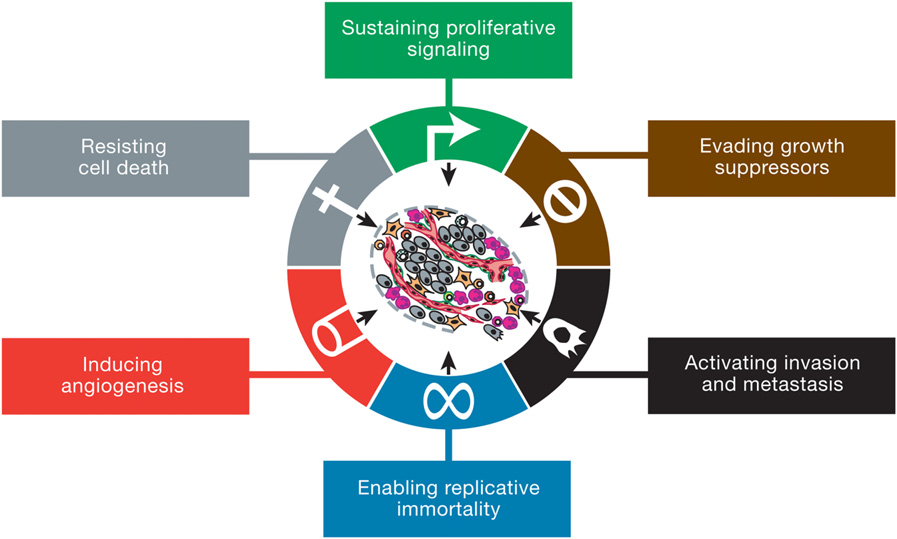
\includegraphics[width=\linewidth]{hanahan_2011_hallmarks.png}\footnotemark
\end{columns}
\footnotetext[1]{\url{https://www.cancer.gov/about-cancer/understanding/statistics}}
\footnotetext[2]{\cite{hanahan_hallmarks_2011}}
\end{frame}

\begin{frame}{Cancer is believed to be caused by somatic mutations}
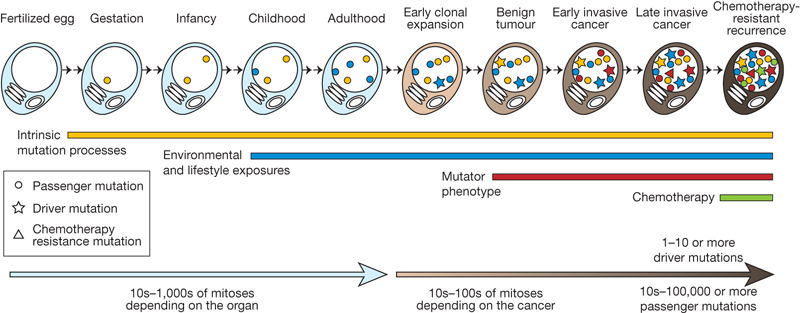
\includegraphics[width=\linewidth]{stratton_2009_mutations.jpg}
\footnotetext[1]{\cite{stratton_cancer_2009}}
\end{frame}

\begin{frame}{Understanding cancer initiation is critical for prevention}
\begin{columns}
\column{.4\textwidth}
\begin{itemize}
\item Some claim Somatic Mutation Theory doesn't explain how sufficient mutations accumulate \parencite{baker_cancer_2015}
\item Disputed evidence that lifetime cancer incidence is linearly correlated with number of somatic cell divisions \parencite{tomasetti_variation_2015}
\end{itemize}
\column{.6\textwidth}
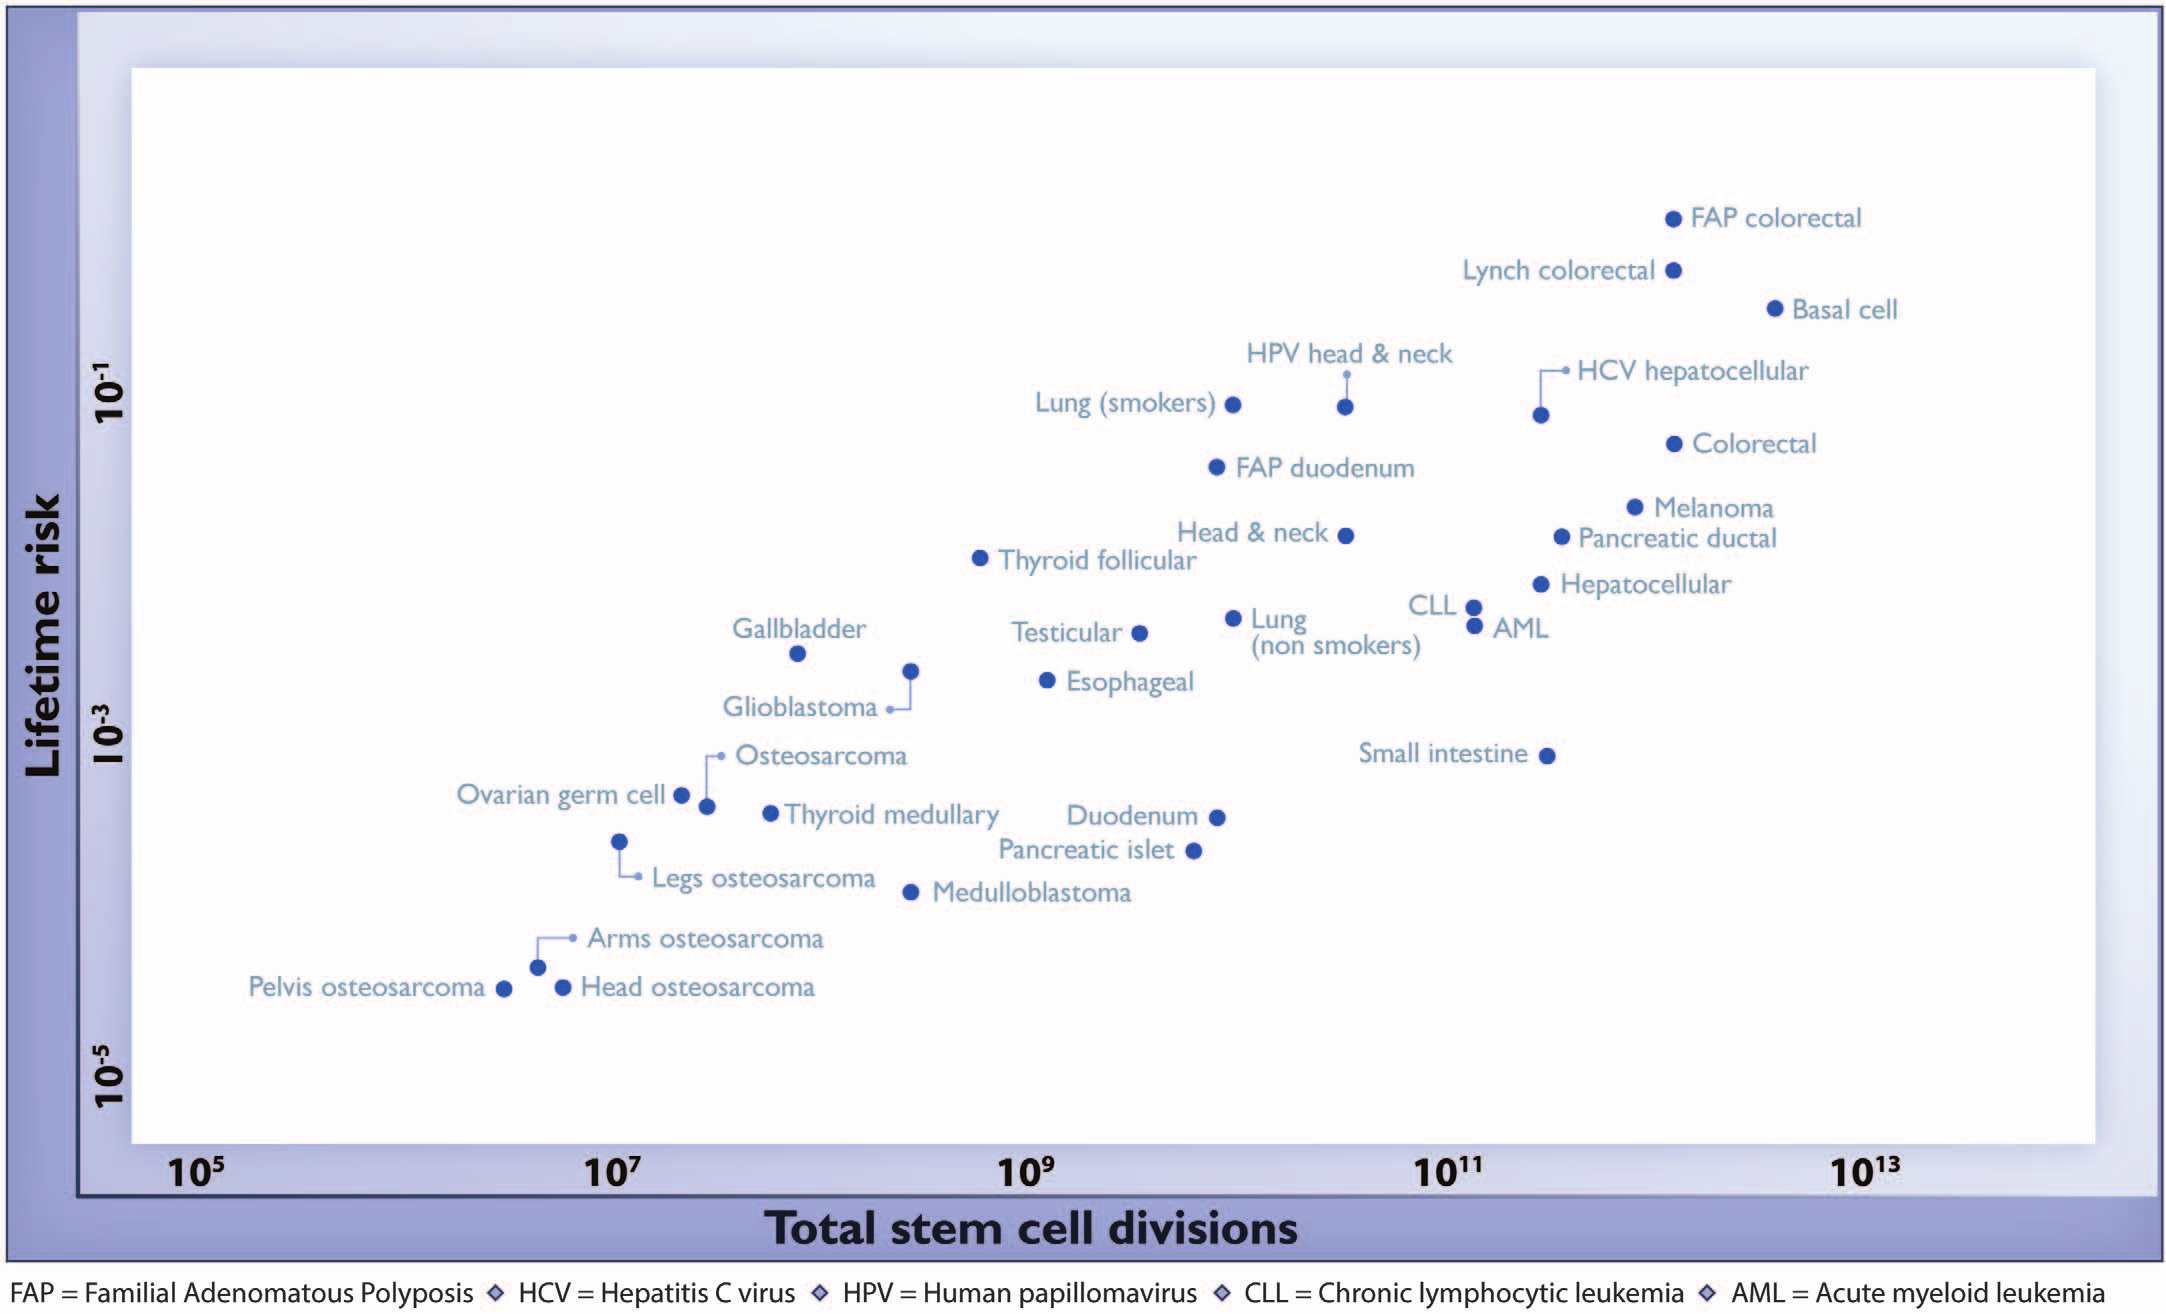
\includegraphics[width=\linewidth]{tomasetti_2015_risk.png}
\end{columns}
\footnotetext[1]{\cite{tomasetti_variation_2015}}
\end{frame}

\begin{frame}{RViMR may explain how so many mutations occur in the correct places}
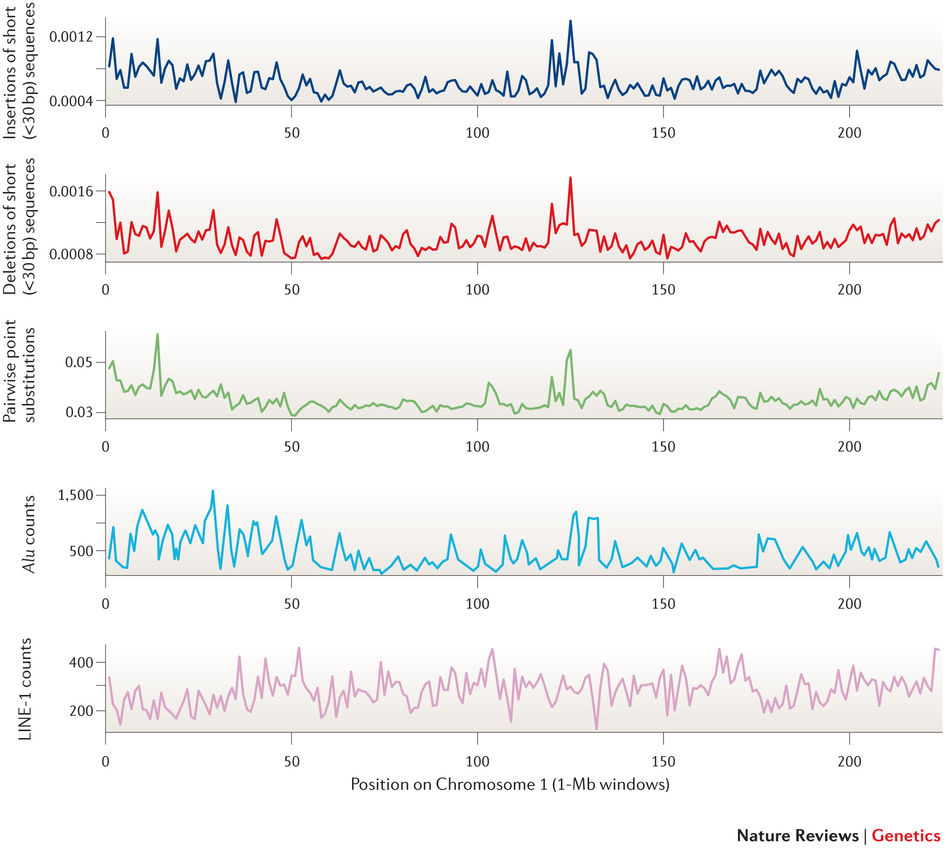
\includegraphics[width=\linewidth,trim={0 13cm 0 0},clip]{makova_2015_rvimr.jpg}
Mutation rates in 1Mb windows across chromosome 1 for different types of mutations \parencite{makova_effects_2015}
\end{frame}

\begin{frame}{Epigenetic markers significantly correlate with local mutation rate}
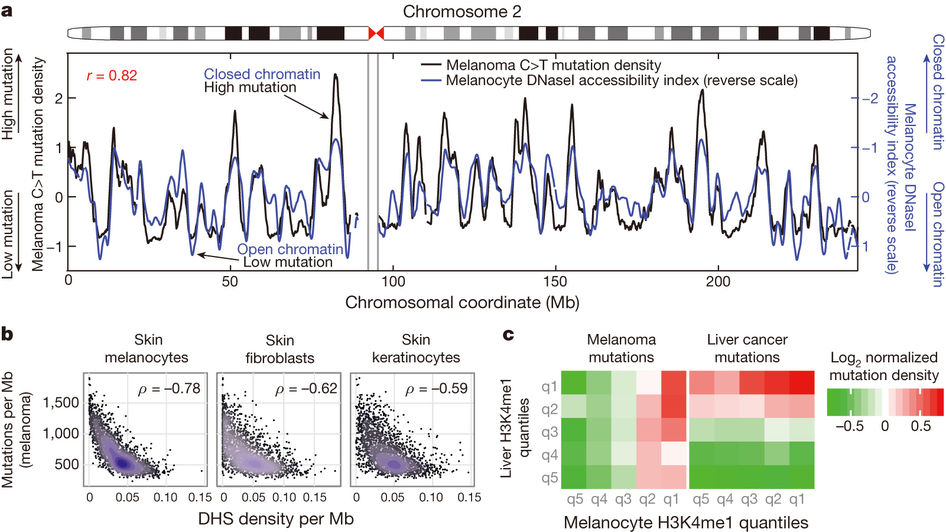
\includegraphics[width=\linewidth,trim={0 7.5cm 0 0},clip]{polak_2015_chromatin.jpg}
\begin{itemize}
\item Closed chromatin regions correlate with high single nucleotide mutation rates. 
\item Open chromatin regions correlate with high insertion/deletion rates \parencite{makova_effects_2015}
\end{itemize}
% \includegraphics[width=\linewidth]{}
\footnotetext[1]{\cite{polak_cell--origin_2015}}
\end{frame}

% \begin{frame}{Nucleosome position and occupancy affect local mutation rate}
% \begin{columns}
% \column{.4\textwidth}
% \column{.6\textwidth}
% % \includegraphics[width=\linewidth]{}
% \end{columns}
% \end{frame}

%how do we study nucleosomes?

\begin{frame}{DNAse-seq}
\begin{columns}
\column{.4\textwidth}
\column{.6\textwidth}
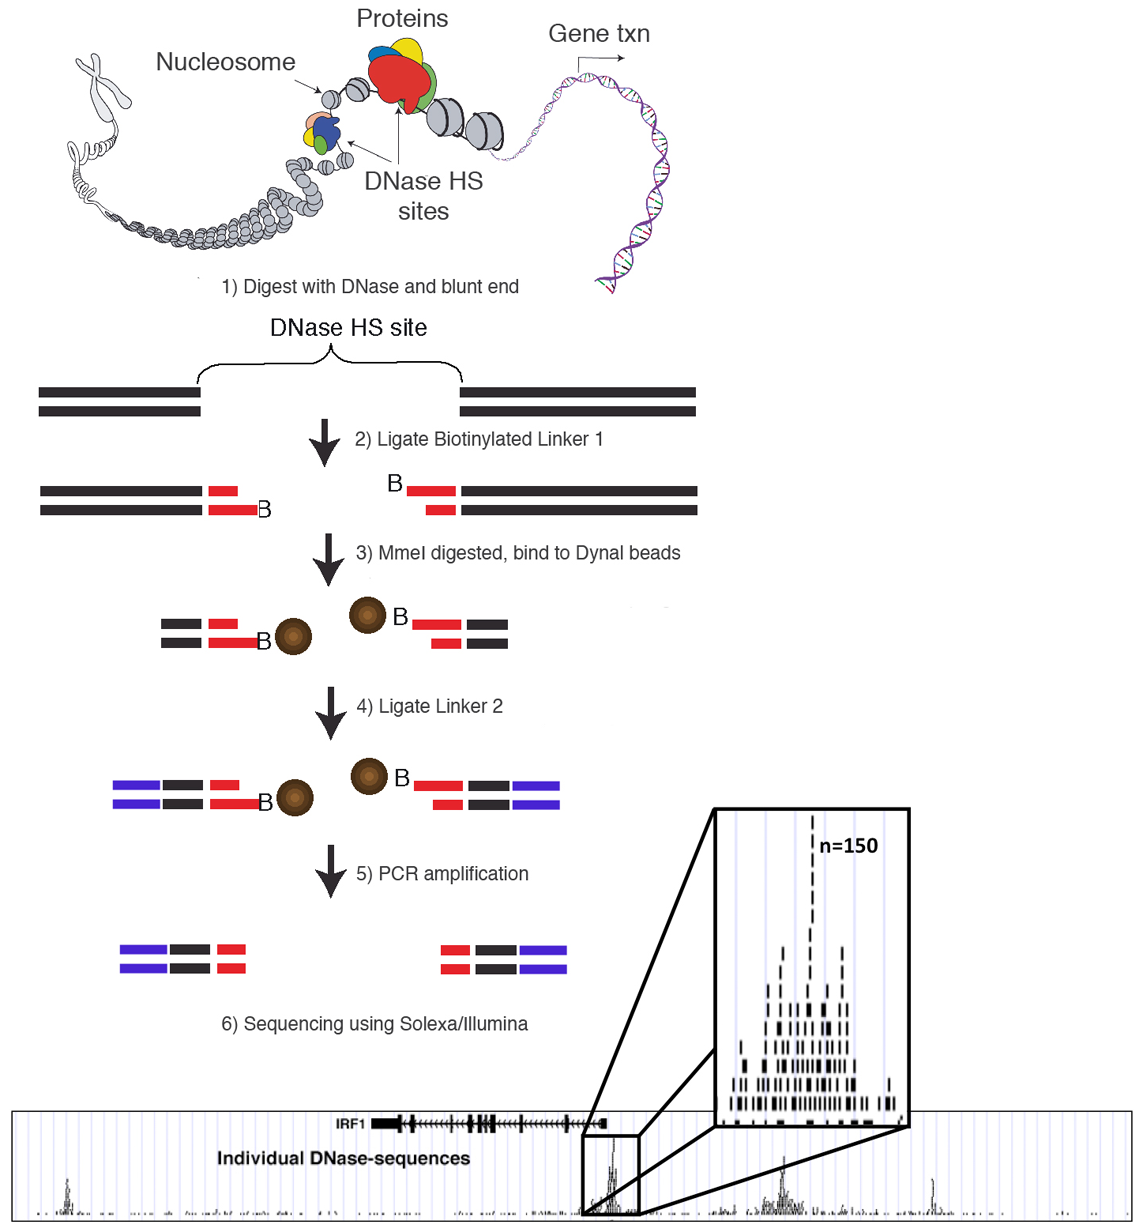
\includegraphics[width=\linewidth]{song_2010_dnase-seq.png}
\footnotetext[1]{\cite{song_dnase-seq:_2010}}
\end{columns}
\end{frame}

% \begin{frame}{ChIP-seq}
% \begin{columns}
% \column{.4\textwidth}
% \column{.6\textwidth}
% % \includegraphics[width=\linewidth]{}
% \end{columns}
% \end{frame}

\begin{frame}{Transposase}
\begin{columns}
\column{.4\textwidth}
\column{.6\textwidth}
% \includegraphics[width=\linewidth]{}
\end{columns}
\end{frame}

\begin{frame}{ATAC-seq}
\begin{columns}
\column{.4\textwidth}
\column{.6\textwidth}
% \includegraphics[width=\linewidth]{}
\end{columns}
\end{frame}

%how do we find mutations?

\begin{frame}{Illumina Sequencing is good for detecting SNPs}
\begin{columns}
\column{.4\textwidth}
\column{.6\textwidth}
% \includegraphics[width=\linewidth]{}
\end{columns}
\end{frame}

\begin{frame}{Nanopore Sequencing is good for detecting insertions and deletions}
\begin{columns}
\column{.4\textwidth}
\column{.6\textwidth}
% \includegraphics[width=\linewidth]{}
\end{columns}
\end{frame}

%what do we need to consider for somatic samples?

\begin{frame}{Heterogeneity is a problem}
\begin{columns}
\column{.4\textwidth}
\column{.6\textwidth}
% \includegraphics[width=\linewidth]{}
\end{columns}
\end{frame}

\begin{frame}{Single cell technology a potential solution, but comes with many more problems}
\begin{columns}
\column{.4\textwidth}
\column{.6\textwidth}
% \includegraphics[width=\linewidth]{}
\end{columns}
\end{frame}

\begin{frame}{Sequencing errors are a problem}
\begin{columns}
\column{.4\textwidth}
\column{.6\textwidth}
% \includegraphics[width=\linewidth]{}
\end{columns}
\end{frame}

\begin{frame}{Reduce number of PCR steps to reduce errors in library prep}
\begin{columns}
\column{.4\textwidth}
\column{.6\textwidth}
% \includegraphics[width=\linewidth]{}
\end{columns}
\end{frame}

\begin{frame}{Read correction reduces errors}
\begin{columns}
\column{.4\textwidth}
\column{.6\textwidth}
% \includegraphics[width=\linewidth]{}
\end{columns}
\end{frame}

\begin{frame}{Small amount of source DNA is a problem}
\begin{columns}
\column{.4\textwidth}
\column{.6\textwidth}
% \includegraphics[width=\linewidth]{}
\end{columns}
\end{frame}

%with all this in mind, our aims!

\begin{frame}{How does chromatin accessibility correlate with mutation rate in the same tissue? How does it change in cancer?}
\begin{columns}
\column{.4\textwidth}
\column{.6\textwidth}
% \includegraphics[width=\linewidth]{}
\end{columns}
\end{frame}

%pipeline stuff
%for the pipeline, do left half text, right half highlight the part of the pipeline we're talking about

\begin{frame}{Pipeline Overview}
\includegraphics[width=\linewidth]{figure.pdf}
\end{frame}

\begin{frame}{Pipeline Validation}
\begin{columns}
\column{.4\textwidth}
\column{.6\textwidth}
% \includegraphics[width=\linewidth]{}
\end{columns}
\end{frame}

\begin{frame}{Short Read Correction - Rcorrector}
\end{frame}

\begin{frame}{Long Read Correction - Nanocorr}
\end{frame}

\begin{frame}{Alignment - Minimap2}
\end{frame}

\begin{frame}{Detect Mutations - MuTect2}
\end{frame}

\begin{frame}{Detect Mutations - Nanopolish}
\end{frame}

\begin{frame}{Calculate Chromatin Accessibility - MACS2}
\end{frame}

\begin{frame}{Tissue Collection}
\end{frame}

\begin{frame}{Library Construction}
\end{frame}

\begin{frame}{Statistical Analysis}
\end{frame}

\begin{frame}{Expected Results - Mutation Rates in Open and Closed Chromatin}
\end{frame}

\begin{frame}{Expected Results - Distribution of Chromatin State at Mutated Sites}
\end{frame}

\begin{frame}{Expected Results - Logistic Regression}
\end{frame}

\begin{frame}{Conclusion}
\end{frame}

\begin{frame}[t, allowframebreaks]
\frametitle{References}
\printbibliography
\end{frame}

\end{document}